\documentclass[a4paper, 12pt]{article}
\usepackage[T2A]{fontenc}
\usepackage[utf8]{inputenc}
\usepackage[english,russian]{babel}
\usepackage{titletoc}
\usepackage{graphicx}
\usepackage{array}
\usepackage{etoolbox}
\usepackage{subfig}
\newcolumntype{P}[1]{>{\centering\arraybackslash}p{#1}}
\def\textunderset#1#2{\leavevmode
  \vtop{\offinterlineskip\halign{%
    \hfil##\hfil\cr\strut#2\cr\noalign{\kern-.3ex}
    \hidewidth\strut#1\hidewidth\cr}}}
\def\signhrule{\raggedright\baselineskip30.0ex \vrule height 0.5pt width30mm depth0pt}

\dottedcontents{section}[2.5em]{\bfseries}{2em}{0.5pc}
\dottedcontents{subsection}[3em]{}{2em}{0.5pc}

\usepackage{listings}
\usepackage{xcolor}

\lstset
{%
		extendedchars=\true,
		frame=tb,
		escapechar=|,
		xleftmargin=0.5cm,
		xrightmargin=0.5cm,
		columns=fullflexible,
		numbers=left,
		numbersep=4pt,
		showspaces=false,
		showstringspaces=false,
		breakatwhitespace=true,
		breaklines=true,
		basicstyle=\color{black}\small\sffamily,
		commentstyle=\color{gray}\itshape,
		stringstyle=\color{orange},
		numberstyle=\footnotesize\color{gray},
		keywordstyle=\color{blue}\bfseries,
		emphstyle={\color{blue}\bfseries},
		tabsize=2,
		texcl=true,
}

\lstloadlanguages{Python, C++}
\newcommand{\Title}{Отчет о выполнении домашней работы}
\newcommand{\TaskType}{домашняя работа}
\newcommand{\SubTitle}{по дисциплине <<Математические методы анализа данных и принятия решений>>}
\newcommand{\LabTitle}{Байесовский классификатор} 
\newcommand{\Faculty}{<<Информатика и системы управления>>}
\newcommand{\Department}{<<Компьютерные системы и сети (ИУ-6)>>}
\newcommand{\AuthorFull}{Козлов Владимир Михайлович}
\newcommand{\Author}{Козлов В.М.}
\newcommand{\Teacher}{}
\newcommand{\group}{ИУ6-13М}
\newcommand{\Year}{2024}
\newcommand{\Country}{Россия}
\newcommand{\City}{Москва}

\newcommand{\UpperFullOrganisationName}{Министерство науки и высшего образования Российской Федерации}
\newcommand{\ShortOrganisationName}{МГТУ~им.~Н.Э.~Баумана}
\newcommand{\FullOrganisationName}{федеральное государственное бюджетное образовательное учреждение высшего профессионального образования\newline <<Московский государственный технический университет имени Н.Э.~Баумана (национальный исследовательский университет)>> (\ShortOrganisationName)}

\textwidth=163mm
\textheight=220mm
\oddsidemargin=-0.5pt
\footskip=30pt
\topmargin=27pt
\headheight=12pt
\headsep=25pt
\topskip=10pt
\baselineskip=15pt
\topmargin=-4mm
\begin{document}
\vspace*{-\baselineskip}
\vspace*{-\headheight}
\vspace*{-\headsep}
\vspace*{-2pt}
\thispagestyle{empty}
\begin{center}

% Шапка
{\centering
\begin{tabular}{P{0.15\textwidth}P{0.85\textwidth}}
\smash{
		\raisebox{-0.9\height}{
		
\includegraphics[width=0.15\textwidth]{includes/bmstu.pdf}
		}}
 & \UpperFullOrganisationName\newline \FullOrganisationName \\
\hline
\multicolumn{1}{p{0.15\textwidth}}{} & \multicolumn{1}{p{0.85\textwidth}}{} \\
\multicolumn{1}{p{0.15\textwidth}}{ФАКУЛЬТЕТ}	&	\multicolumn{1}{p{0.85\textwidth}}{\Faculty}	\\
\multicolumn{1}{p{0.15\textwidth}}{КАФЕДРА}	&	\multicolumn{1}{p{0.85\textwidth}}{\Department}	\\
\end{tabular}}
\vfil

{% Основная часть
\vfil
\Large
\underline{\MakeUppercase{\Title}}
\newline
\SubTitle
\vfil
\large
\begin{tabular}{p{0.3\textwidth}p{0.5\textwidth}} 
	Студент:	& \AuthorFull \\ 
	\hline
	Группа:	& \group \\ 
	\hline
	Тип задания:	& \TaskType \\ 
	\hline
	Тема:	& \LabTitle \\ 
	\hline
	\end{tabular}

\vfil

\begin{tabular}{p{0.45\textwidth}p{0.25\textwidth}P{0.25\textwidth}} 
\large
Студент	&	\textunderset{\scriptsize{подпись, дата}}{\signhrule} & \textunderset{\scriptsize{Фамилия, И.О.}}{\ifdefempty{\Author}{\signhrule}{\underline{\Author}}} \\ 
& & \\
Преподаватель	&	\textunderset{\scriptsize{подпись, дата}}{\signhrule} & \textunderset{\scriptsize{Фамилия, И.О.}}{\ifdefempty{\Teacher}{\signhrule}{\underline{\Teacher}}} \\ 
\end{tabular}
}

\vfil
\vfil
\City, \Year

\end{center}

\pagebreak
\tableofcontents
\newpage
% Основная часть --------------------------------------------------------------------------------------------
\section*{Задание}
\addcontentsline{toc}{section}{Задание}
Сюда задание.

\newpage
% -------------------------------------------------------
\section{Заголовок}
\subsection{Подзаголовок}
Пример цитаты.\cite{ALT}
\begin{center}
    \centering
    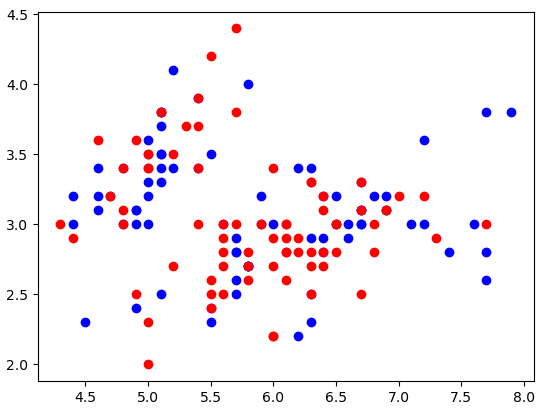
\includegraphics[width=.7\linewidth]{extras/output.png}
    \captionof{figure}{Картинка}
    \label{fig:prplot}
\end{center}
\begin{lstlisting}[language=Python, caption=листинг]
    print("Hello world!")
\end{lstlisting}

\lstinputlisting[style=text, caption=вставка текста файла]{extras/table.csv}

\begin{table}
    \centering
    \csvautotabular{extras/table.csv}
\caption{Вставка таблицы из файла}
\end{table}
%---------------------------------------------
\newpage
\bibliographystyle{includes/utf8gost705u}

\section*{Список использованных источников}
\addcontentsline{toc}{section}{Список использованных источников}

\begingroup
\renewcommand{\section}[2]{}%
%\renewcommand{\chapter}[2]{}% for other classes
\bibliography{citations}
\endgroup

\bibentry{ALT}
\bibentry{KafkaDocumentation}

\end{document}

